\chapter{Bond Market}
\section{Introduction}

\begin{definitionbox}{Bond Definition}
    A bond is a certificate issued by a company to raise funds akin to a loan, where it will pay back the principal amount at a specified date, and pay interest at a specified rate.
\end{definitionbox}

Bonds represent a type of security. Like all securities, there must be a legal document that outlines the terms and conditions of the bond. This legal document is called the \textbf{bond indenture}.

\subsection*{Typical Parts of a Bond Indenture}
\begin{itemize}
    \item \textbf{Bond Details}
    \begin{itemize}
        \item Face value or principal amount of the bond
        \item Interest rate, also called the coupon rate payable to bondholders
        \item Maturity date
        \item Any provisions for early redemption or call options
\begin{sidenotebox}{More info on early redemption and call options}
    \begin{itemize}
        \item Callable bonds can be redeemed by the issuer before the maturity date, i.e. the issuer has the right (not obligation) to repay the principal amount before the maturity date.
        \item Puttable bonds can be sold back to the issuer before the maturity date, i.e. the holder of the puttable bond has the right (not obligation) to demand the early repayment of the principal amount.
    \end{itemize}
\end{sidenotebox}
    \end{itemize}
    \item \textbf{Payment Terms}
    \begin{itemize}
        \item Outline the timing and method of interest payments to bondholders
        \item Determines if payments are made periodically (coupon bonds) or as a lump sum at maturity (zero-coupon bonds)
    \end{itemize}
    \item \textbf{Covenants}
    \begin{itemize}
        \item Includes clauses and restrictions to protect bondholders' interests
        \item Example: provisions on issuer's ability to issue more debt
        \item Example: restrictions on the issuer maintaining certain financial ratios
        \item Example: Restricting asset sales or limiting dividend payments
    \end{itemize}
    \item \textbf{Collateral/Security}
    \begin{itemize}
        \item Specifies nature and value of the collateral
        \item Collateral is an asset that the issuer pledges to the bondholders to secure the bond
        \item If the issuer defaults, bondholders can seize the collateral to recover their investment
    \end{itemize}
    \item \textbf{Defaults and Remedies}
    \begin{itemize}
        \item Outlines the conditions under which the issuer is considered in default
        \item Specifies the remedies available to bondholders in case of default
        \item Example: Acceleration clause allows bondholders to demand immediate repayment if the issuer defaults
        \item Example: Appointment of a trustee to represent bondholders' interests, this could mean the trustee can take control of the issuer's assets to repay bondholders
    \end{itemize}
\end{itemize}

\subsection*{Face Value}
The face value of a bond is the notional value or amount that bondholders have lent to the issuer company. The issuer agrees to repay the bondholder this amount at maturity. It is also called the \textbf{par value} or \textbf{principal amount}.

\subsection*{Bond Term}
The term of the bond refers to the duration for which the money has been lent, or the time until the bond reaches maturity.

\subsection*{Payment Terms}
\begin{itemize}
    \item \textbf{Coupon Bonds:} These bonds pay interest to bondholders at regular intervals, typically semi-annually or annually. The interest payment is called the \textbf{coupon payment}. Then at maturity, the bondholder receives the face value of the bond.
    \item \textbf{Zero-Coupon Bonds:} These bonds do not pay interest to bondholders. Instead, they are issued at a discount to the face value, and the bondholder receives a single cash flow equal to the face value at maturity.
\end{itemize}

\begin{definitionbox}{UK Goverment Debt}
    The Debt Management Office (DMO) is responsible for managing the UK government's debt. The DMO issues gilts, which are UK government bonds. Gilts are considered to be risk-free assets, as the UK government is unlikely to default on its debt.
\end{definitionbox}

\section{The Law of One Price}
The law of one price states that identical goods should sell for the same price in different markets. This principle applies to bonds, where two bonds with the same risk and cash flows should sell for the same price.


\subsection*{Government Debt (Sovereign Bonds)}
\begin{itemize}
    \item It is generally assumed that governments honour their debt obligations, so government bonds are considered risk-free.
    \item This simplifies the valuation of government bonds, as we assume that we can exclude considerations of credit risk, the possibility of default.
    \item \textbf{Zero-Coupon Bonds} are the simplest type, often called zeros. They are sold at a discount to the face value, and the bondholder receives the face value at maturity. There are no coupon payments.
    \begin{itemize}
        \item It is simple to calculate the price of a zero-coupon bond, as there are only two cash flows: the purchase price and the face value.
        \item The investor pays a price $P$ for the bond to the government.
        \item The government pays the face value $FV$ to the investor at maturity
        \item Since the initial price $P$ is discounted from $FV$, we define the interest rate, or yield to maturity, $r$ as the rate that equates the present value of the face value to the price paid, over $N$ periods.
        \item The yield to maturity represents the average return over the bond's term for the investor.
        \item We have the formulas:
        \begin{equation}
               P = \frac{FV}{(1 + r)^N}
              \end{equation}
        \begin{equation}
                r = \left(\frac{FV}{P}\right)^{\frac{1}{N}} - 1
        \end{equation}
    \end{itemize}
    \item \textbf{Coupon Bonds} involve regular coupon payments to bondholders, in addition to the face value at maturity. A coupon payment is referred to as $C$. 
    \begin{equation}
        C = \frac{\text{Coupon Rate} \times FV}{\text{Number of interest payments per year}}
    \end{equation}
    \item The price of a coupon bond is the sum of the present value of the coupon payments and the present value of the face value, where $N$ is the number of periods until maturity. 
        \begin{align}
            P &= \sum_{t=1}^{N} \frac{C}{(1 + r)^t} + \frac{FV}{(1 + r)^N}\\
              &\equiv C \times \frac{ 1-(1+ r)^{-N}}{r} + \frac{FV}{(1 + r)^N}
          \end{align}
    \item In the second line, the geometric sum formula is used to simplify the sum of the coupon payments.
    \item It is easy to see that the current price of a bond is inversely related to the yield to maturity. If the yield to maturity increases, the bond price decreases, and vice versa.
    \item This is because when yield to maturity increases, fewer people want to buy a bond with a coupon rate that is relatively lower than the yield to maturity (they will prefer a bond with a higher coupon rate to offset the increased yield to maturity).
    \item Another attribute of a bond is its current yield, which is the annual coupon payment divided by the bond's price.
    \begin{equation}
        \text{Current Yield} = \frac{\text{Annual Rate}}{P} = \frac{\text{Coupon Rate} \times FV}{P}
    \end{equation}
        
\end{itemize}

\subsection*{Examples of the Law of One Price}
\subsubsection*{Bonds vs Deposit}
\begin{itemize}
    \item Assume interest rates are constant, and are expected to remain so at say, 5\%.
    \item Consider a coupon-paying bond with coupons equal to 5\% of the face value.
    \item The bond would be selling at par, meaning its price equals its face value.
    \item The coupon payments are then directly equivalent to interest payments, and the final redemption payment is the face value.
    \item Investing in the bond would provide the same return as a deposit account paying 5\% interest, with the same cash flows.
    \item Therefore, the bond's price and the deposit account's value should be the same due to the law of one price.
\end{itemize}

\subsubsection*{Two Government Bonds}
\begin{itemize}
    \item Consider a French bond and a German bond, both denominated in Euros.
    \item In a well-functioning market, we would assumedly expect the returns from lending to the French government to be approximately the same as lending to the German government.
    \item Therefore, we would not expect a significant difference in yield to maturity on the average interest rate paid by each government.
    \item If there was a large disparity in returns under normal market conditions, investors would prefer the bond offering the higher return.
    \item This would lead to increased demand for that bond, causing its price to rise and its yield to decrease until it reaches a level equal to the other bond.
    \item In an efficient market, comparable bonds with similar risk profiles would have equal yields to maturity, which can be seen as the market interest rate for that bond's term. 
    \item Consequently, we can refer to the yield to maturity of a two-year zero as the interest rate on two-year money, without distinguishing the specific instrument, as an efficient market would have similar rates across different types of bonds.
\end{itemize}

\begin{examplebox}{Coupon Bond Calculation Questions}
\textbf{Question 1:} A bond has a 7\% coupon and pays interest semi-annually. What is the amount of each interest payment if the face value of a bond is \pounds100?

\textbf{Answer:}
The interest payment, or coupon payment, for a bond can be calculated using the formula:
\[ \text{Interest payment} = \frac{\text{Coupon rate} \times \text{Face amount}}{\text{Number of interest payments per year}} \]

For a 7\% coupon rate with semi-annual payments:
\[ = \frac{0.07 \times \pounds100}{2} \]
\[ = \frac{\pounds7}{2} \]
\[ = \pounds3.50 \]

\textbf{Question 2:} A bond has a 9\% coupon rate, matures in three years, and pays interest semi-annually. The face value is \pounds100. What is the current price of this bond if the market rate of return is 8.3\%?

\textbf{Answer:}
The current price of the bond can be calculated using the present value of future cash flows. The formula for the bond price using the longhand method is:
\[ P = \frac{C}{(1+r)} + \frac{C}{(1+r)^2} + \cdots + \frac{C + FV}{(1+r)^t} \]

Where \( C \) is the coupon payment, \( FV \) is the face value, \( r \) is the market rate of return per period, and \( t \) is the total number of periods.

Given a 9\% coupon rate, with semi-annual payments and a market rate of return of 8.3\%, the bond price is:
\begin{align*} P &= \frac{\pounds4.5}{(1.0415)}  +  \frac{\pounds4.5}{(1.0415)^2} + \cdots + \frac{\pounds104.5}{(1.0415)^6} \\
&=\left(\frac{0.09\times£100}{2}\times\frac{1-\left[\frac{1}{\left(1+\frac{0.083}{2}\right)^{3\times2}}\right]}{\frac{0.083}{2}}\right)+\frac{£100}{\left(1+\frac{0.083}{2}\right)^{3\times2}}
\end{align*}
\[ = \pounds101.83 \]

The shorthand method for the bond price is:
\[ P = \left( CPN \times \left[ \frac{1 - \left[ \frac{1}{(1+r)^t} \right]}{r} \right] \right) + \frac{FV}{(1+r)^t} \]
\[ = \pounds101.83 \]

\textbf{Question 3:} An 8\%, semi-annual coupon bond has a \$1000 face value and matures in eight years. What is the current yield on this bond if the yield to maturity is 7.8\%?

\textbf{Answer:}
The current yield is calculated as:
\[ \text{Current yield} = \frac{\text{Annual yield}}{\text{Current price}} \]

We first calculate the current price:

\begin{align*}
    P&=\left(CPN\times\left(\frac{1-\left[\frac1{\left(1+r\right)^{t}}\right]}{r}\right)\right)+\frac{FV}{\left(1+r\right)^{t}} \\
    P&=\left(\frac{0.08\times1000}{2}\times\left(\frac{1-\left[\frac{1}{(1+\frac{0.078}{2})^{8\times2}}\right]}{\frac{0.078}{2}}\right)\right)+\frac{1000}{\left(1+\frac{0.078}{2}\right)^{8\times2}} \\
    &=(\$40\times11.73873)+\$542.18967 \\
    &=\$469.54920+\$542.18967 \\
    &=\$1,011.74
\end{align*}

For an 8\% coupon rate with a \$1000 face value and a yield to maturity of 7.8\%:
\[ = \frac{\$80}{\$1011.74} \]
\[ = 0.07907 \]
\[ = 7.91\% \]
\end{examplebox}

\renewcommand{\thesection}{2.3 - 2.4}
\section{Yield Curves}
\setcounter{section}{4}
\renewcommand{\thesection}{\arabic{chapter}.\arabic{section}}

A yield curve is a representation of how the market expects interest rates to vary in the future.

It shows the relationship between the yield to maturity and the time to maturity for a set of similar bonds. The following diagram shows a typical yield curve for zero-coupon bonds.

\begin{figure}[H]
    \centering
    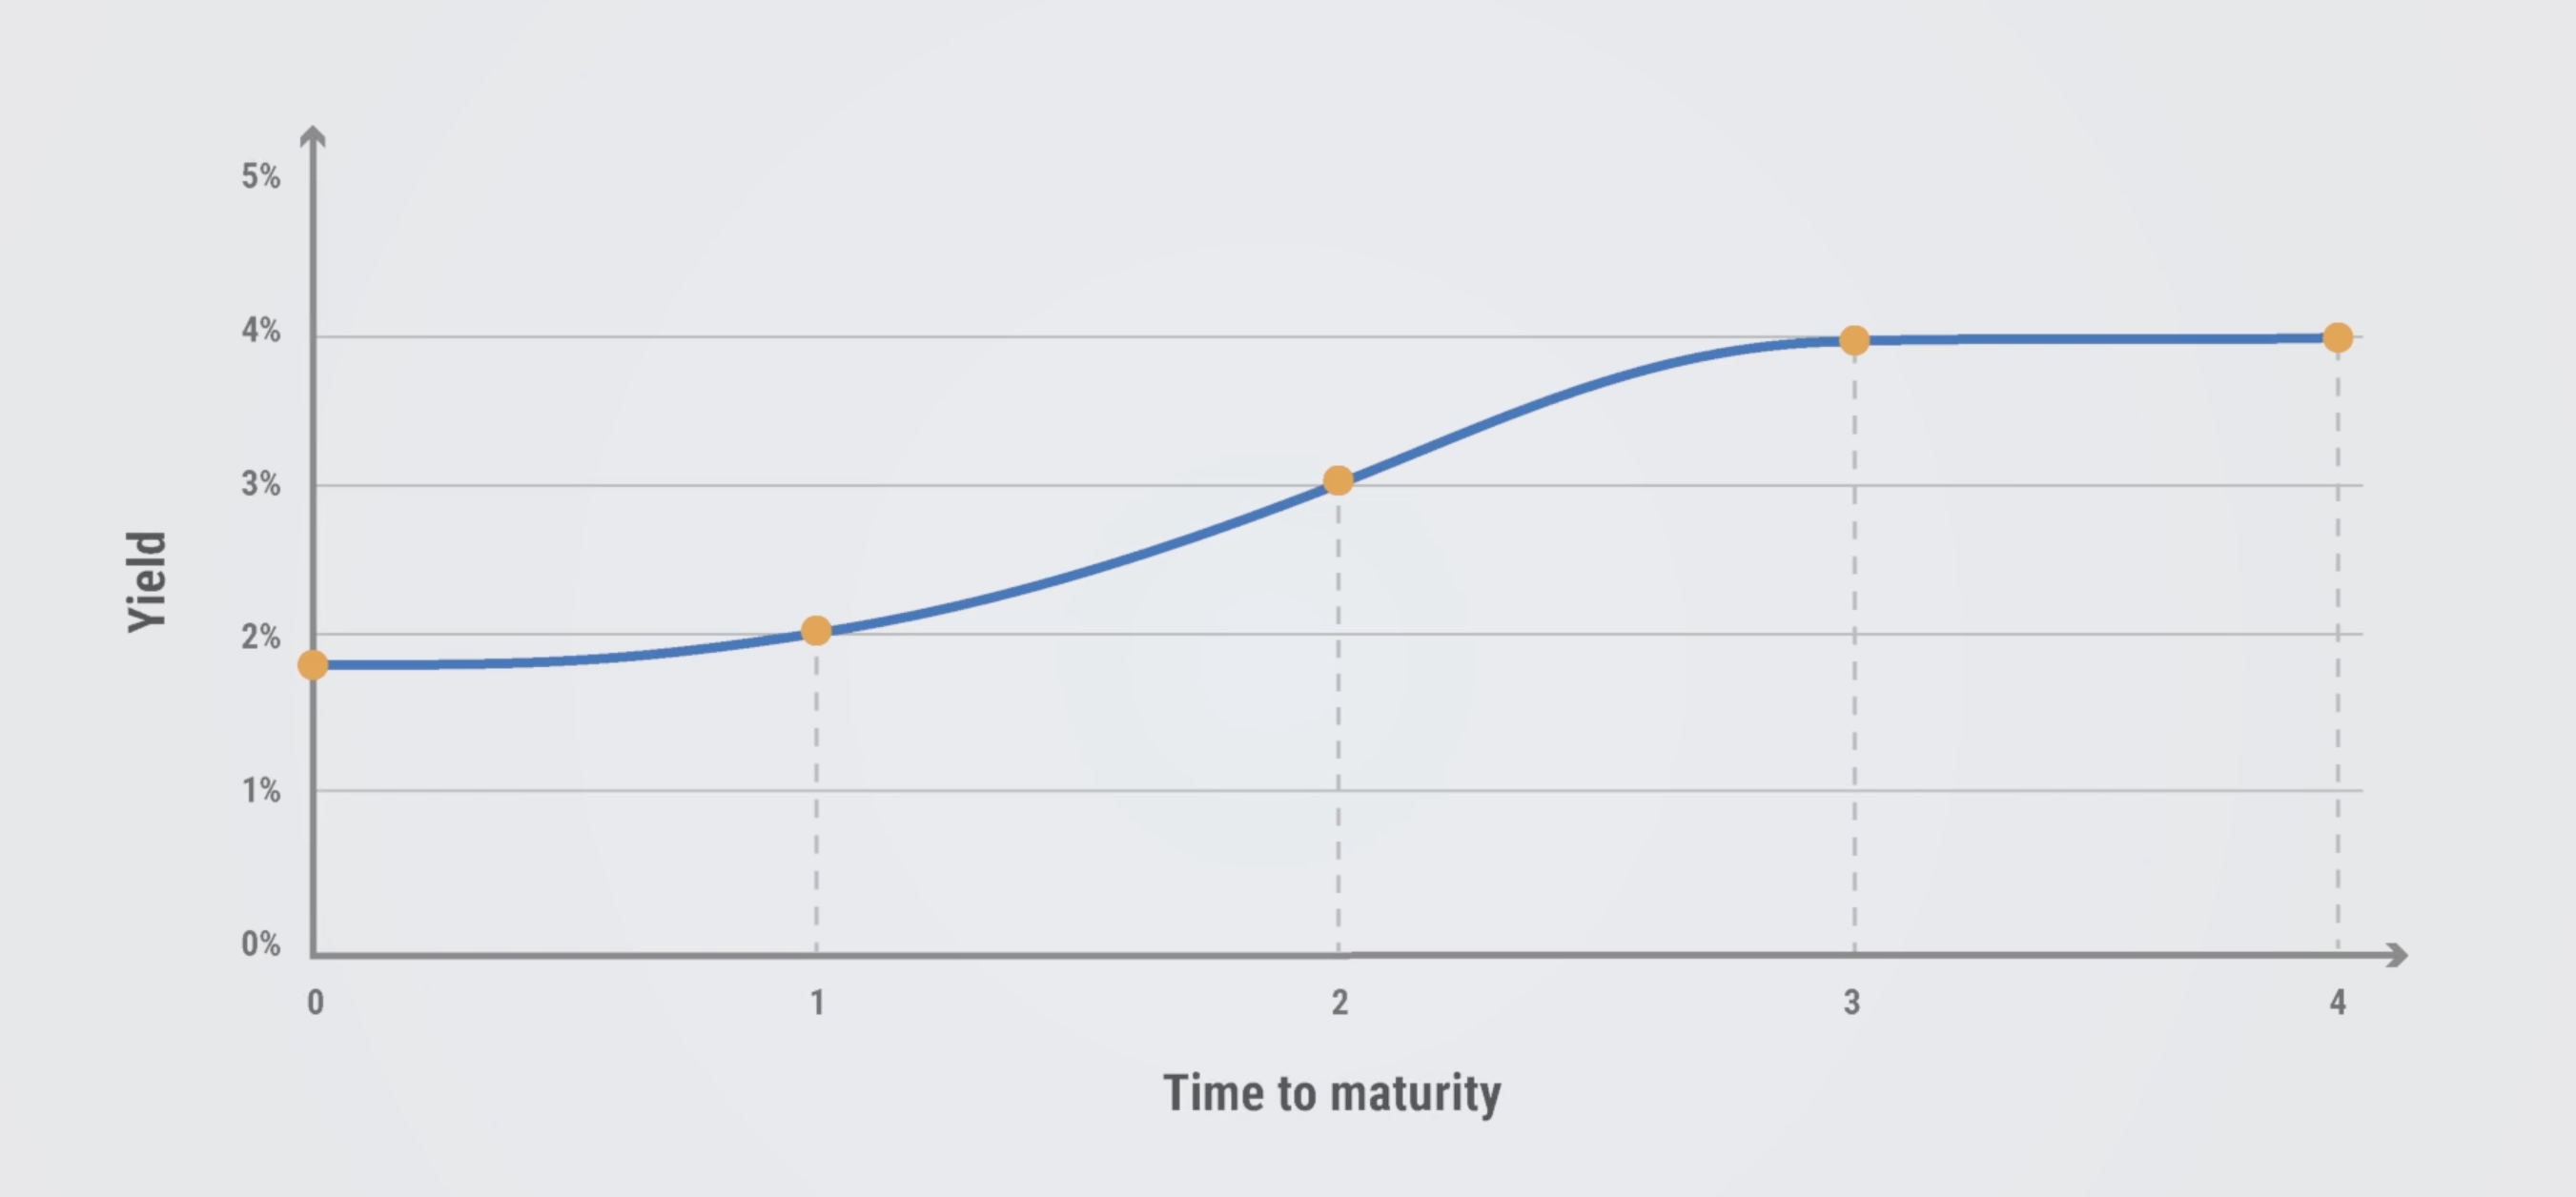
\includegraphics[width=0.8\textwidth]{img/2.1.png}
    \caption{Yield Curve for Zero-Coupon Bonds}
    \label{fig:yield_curve}
\end{figure}

The yield for a one-year zero-coupon bond is 2\%, for a two-year bond it is 3\%, and for a three-year bond it is 4\%. This is an example of a normal yield curve, where longer-term bonds have higher yields than shorter-term bonds. \\


There is a gradual increase in interest rates as the time to maturity increases, but this does not always hold. In this case, the increase tapers off at 5\%, for a four-year bond. This is known as the \textbf{flattening} of the yield curve, and that the markets expect interest rates to remain stable in the long term.

\section{Pricing Coupon Bonds with the Yield Curve}

It is trivial to price coupon bonds with a variable rate determined by the yield curve. 

Using the example yield curve in Figure \ref{fig:yield_curve}, and assuming round numbers for simplicity, we have:

\begin{table}[htbp]
    \centering
    \caption{Yield Curve for Zero-Coupon Bonds}
    \label{tab:yield_curve}
    \begin{tabular}{@{} c c c @{}}
    \toprule
    \textbf{Time to Maturity} & \textbf{Yield to Maturity} & \textbf{Discounted Payment} \\
    \midrule
    1 year & 2\% & ${5}/{(1+0.02)^1}$\\
    2 years & 3\% & ${5}/{(1+0.03)^2}$\\
    3 years & 4\% & ${5}/{(1+0.04)^3}$\\
    4 years & 4\% & ${(5+100)}/{(1+0.04)^4}$\\  
    \bottomrule
    \end{tabular}
\end{table}

Where the last payment includes the face value of the bond.\\

To price a four-year coupon bond with a 5\% coupon rate for the face value of £100 with annual payments, this will be a £5 coupon payment in years 1-3, followed by a £105 payment in year 4.\\

We thus have the following for the fair price of the bond:

\[
P = \frac{5}{(1+0.02)^1} + \frac{5}{(1+0.03)^2} + \frac{5}{(1+0.04)^3} + \frac{105}{(1+0.04)^4}  = 103.8
\]
\renewcommand{\thesection}{2.6 - 2.8}
\section{Yield Curve (Live Class)}
\setcounter{section}{8}
\renewcommand{\thesection}{\arabic{chapter}.\arabic{section}}

\subsection*{The Company's Balance Sheet}

\begin{figure}[H]
    \centering
    \begin{tikzpicture}
        % Define the styles for each block
        \tikzstyle{block} = [rectangle, draw, fill=blue!30, text width=14em, text centered, minimum height=9em, inner sep=0, outer sep = 0]
        \tikzstyle{blockgreen} = [rectangle, draw, fill=green!30, text width=14em, text centered, minimum height=6em, inner sep=0, outer sep = 0]

        % Define the nodes for Current Assets and Fixed Assets
        \node[block] (current) {Current Assets};
        \node[block, below=0 of current] (fixed) {Fixed Assets\\Tangible\\Intangible};

        % Calculate the total height of the left blocks (current and fixed)
        \path let \p1 = ($(current.north)-(fixed.south)$), \n1 = {veclen(\y1,\x1)} in -- (current.north east) coordinate (middlepoint);

        % Define the nodes for Current Liabilities, Long-Term Debt, and Shareholders' Equity
        % Adjust the heights to account for the borders of the nodes
        \node[blockgreen, below=0 of middlepoint, anchor=north west, ] (currentliab) {Current Liabilities};
        \node[blockgreen, below=0 of currentliab.south west, anchor=north west, ] (longterm) {Long-Term Debt};
        \node[blockgreen, below=0 of longterm.south west, anchor=north west, ] (equity) {Shareholders' Equity};
    
    \end{tikzpicture}
    \caption{Simplified diagram graphic of the Company Balance Sheet.}
    \label{fig:balance_sheet}
\end{figure}

The table in Figure \ref{fig:balance_sheet} shows a simplified version of a company's balance sheet. Current assets could refer to cash, inventory, or accounts receivable. Fixed assets could refer to property, manufacturing plants, and equipments. Current liabilities could refer to accounts payable, short-term loans, or taxes payable. Long-term debt could refer to bonds or loans with a maturity of more than one year. 

Figure \ref{fig:balance_sheet} also shows the fundamental accounting equation: 
\begin{equation}
    \text{Assets} = \text{Liabilities} + \text{Equity}
\end{equation}

Which is rewritten as:
\begin{equation}
    \text{Equity} = \text{Assets} - \text{Liabilities}
\end{equation}

This simply means that shareholders own all of the assets minus liabilities, i.e. the company's equity is the residual value of the company's assets after all liabilities have been paid off.\\

\subsection*{Capital Budgeting Decision}

We take the previous table from Figure \ref{fig:balance_sheet} and simplify it further:

\begin{figure}[H]
    \centering
    \begin{tikzpicture}
        % Define the styles for blocks and labels
        \tikzstyle{block} = [rectangle, draw, fill=blue!30, text width=14em, text centered, minimum height=9em, inner sep=0, outer sep = 0]
        \tikzstyle{block2} = [rectangle, draw, fill=blue!30, text width=14em, text centered, minimum height=3em, inner sep=0, outer sep = 0]
        \tikzstyle{blockgreen} = [rectangle, draw, fill=green!30, text width=14em, text centered, minimum height=6em, inner sep=0, outer sep = 0]
        \tikzstyle{labelstyle} = [rectangle, text width=14em, text centered, inner sep=0, outer sep = 0]

        % Labels for the columns
        \node[labelstyle] (label1) at (0em,0em) {Invested Capital};
        \node[labelstyle] (label2) at (14em,0em) {Equity and Debt};
        

    
        \path let \p1 = (label1.south), \p2 = (current.north) in [yshift=(\y1-\y2)] node[labelstyle] at (current.north) {};

        % Define the nodes for Current Assets and Fixed Assets
        \node[block2, below=of label1] (current) {Net Working Capital = C. Assets $-$ C. Liabilities};
        \node[block, below=0 of current] (fixed) {Fixed Assets\\Tangible\\Intangible};

        % Calculate the total height of the left blocks (current and fixed)
        \path let \p1 = ($(current.north)-(fixed.south)$), \n1 = {veclen(\y1,\x1)} in -- (current.north east) coordinate (middlepoint);

        % Define the nodes for Long-Term Debt, and Shareholders' Equity
        \node[blockgreen, below=of label2] (longterm) {Long-Term Debt};
        \node[blockgreen, below=0 of longterm] (equity) {Shareholders' Equity};


    \end{tikzpicture}
    \caption{Processed diagram graphic of the Company Balance Sheet.}
    \label{fig:balance_sheet_2}
\end{figure}


This operation now defines the left column as invested capital. It is used to ask what long-term investments that the firm should choose to maximise value. The right column is equity and debt, which is used to ask how the firm should finance these investments.\\

The value of the firm can be thought of as a pie:

\begin{figure}[H]
    \centering
    \begin{subfigure}{0.4\textwidth}
        \centering
        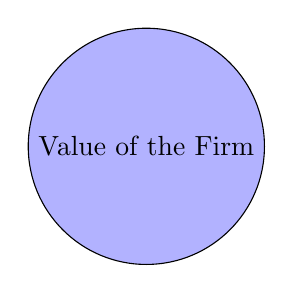
\begin{tikzpicture}
            \draw[fill=blue!30] (0,0) circle (1.5cm) node[midway] {Value of the Firm};
        \end{tikzpicture}
        \caption{Value Composition}
        \label{fig:value_firm1}
    \end{subfigure}
    \begin{subfigure}{0.4\textwidth}
        \centering
        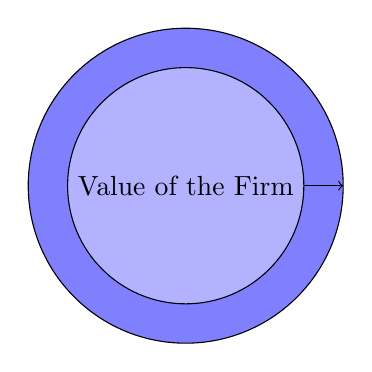
\begin{tikzpicture}
            \draw[fill=blue!50] (0,0) circle (2cm) node[midway] {};
            \draw[fill=blue!30] (0,0) circle (1.5cm) node[midway] {Value of the Firm};
            \draw[fill=black, ->] (1.5cm,0) -- (2.0,0cm) node[midway, yshift=0.5cm] {};
        \end{tikzpicture}
        \caption{Value Composition Increased}
        \label{fig:value_firm2}
    \end{subfigure}
    \caption{Goal: increase pie size }
    \label{fig:value_firm}
\end{figure}

The role of the manager is to increase the size of the pie's net present value. The Capital Structure decision can be viewed as how best to slice the pie.

\begin{figure}[H]
    \centering
    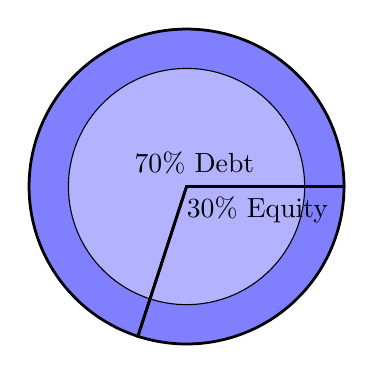
\begin{tikzpicture}
        % Draw the filled circles
        \draw[fill=blue!50] (0,0) circle (2cm); % Outer circle
        \draw[fill=blue!30] (0,0) circle (1.5cm) node[midway] {}; % Inner circle

        % Add the arcs for the pie chart on top
        % Outline of 70% Debt arc
        \draw[line width=1pt] (0,0) -- (2cm,0) arc (0:252:2cm) -- cycle;
        % Outline of 30% Equity arc
        \draw[line width=1pt] (0,0) -- (2cm,0) arc (0:-108:2cm) -- cycle;
        
        % Labels for Debt and Equity
        \node at (0.1cm,0.3cm) {70\% Debt};
        \node at (0.9cm,-0.3cm) {30\% Equity};
    \end{tikzpicture}
    \caption{The capital structure decision slices the pie.}
    \label{fig:debt_equity_circle}
\end{figure}

\subsection*{The Role of Financial Markets}

\begin{figure}[H]
    \centering
    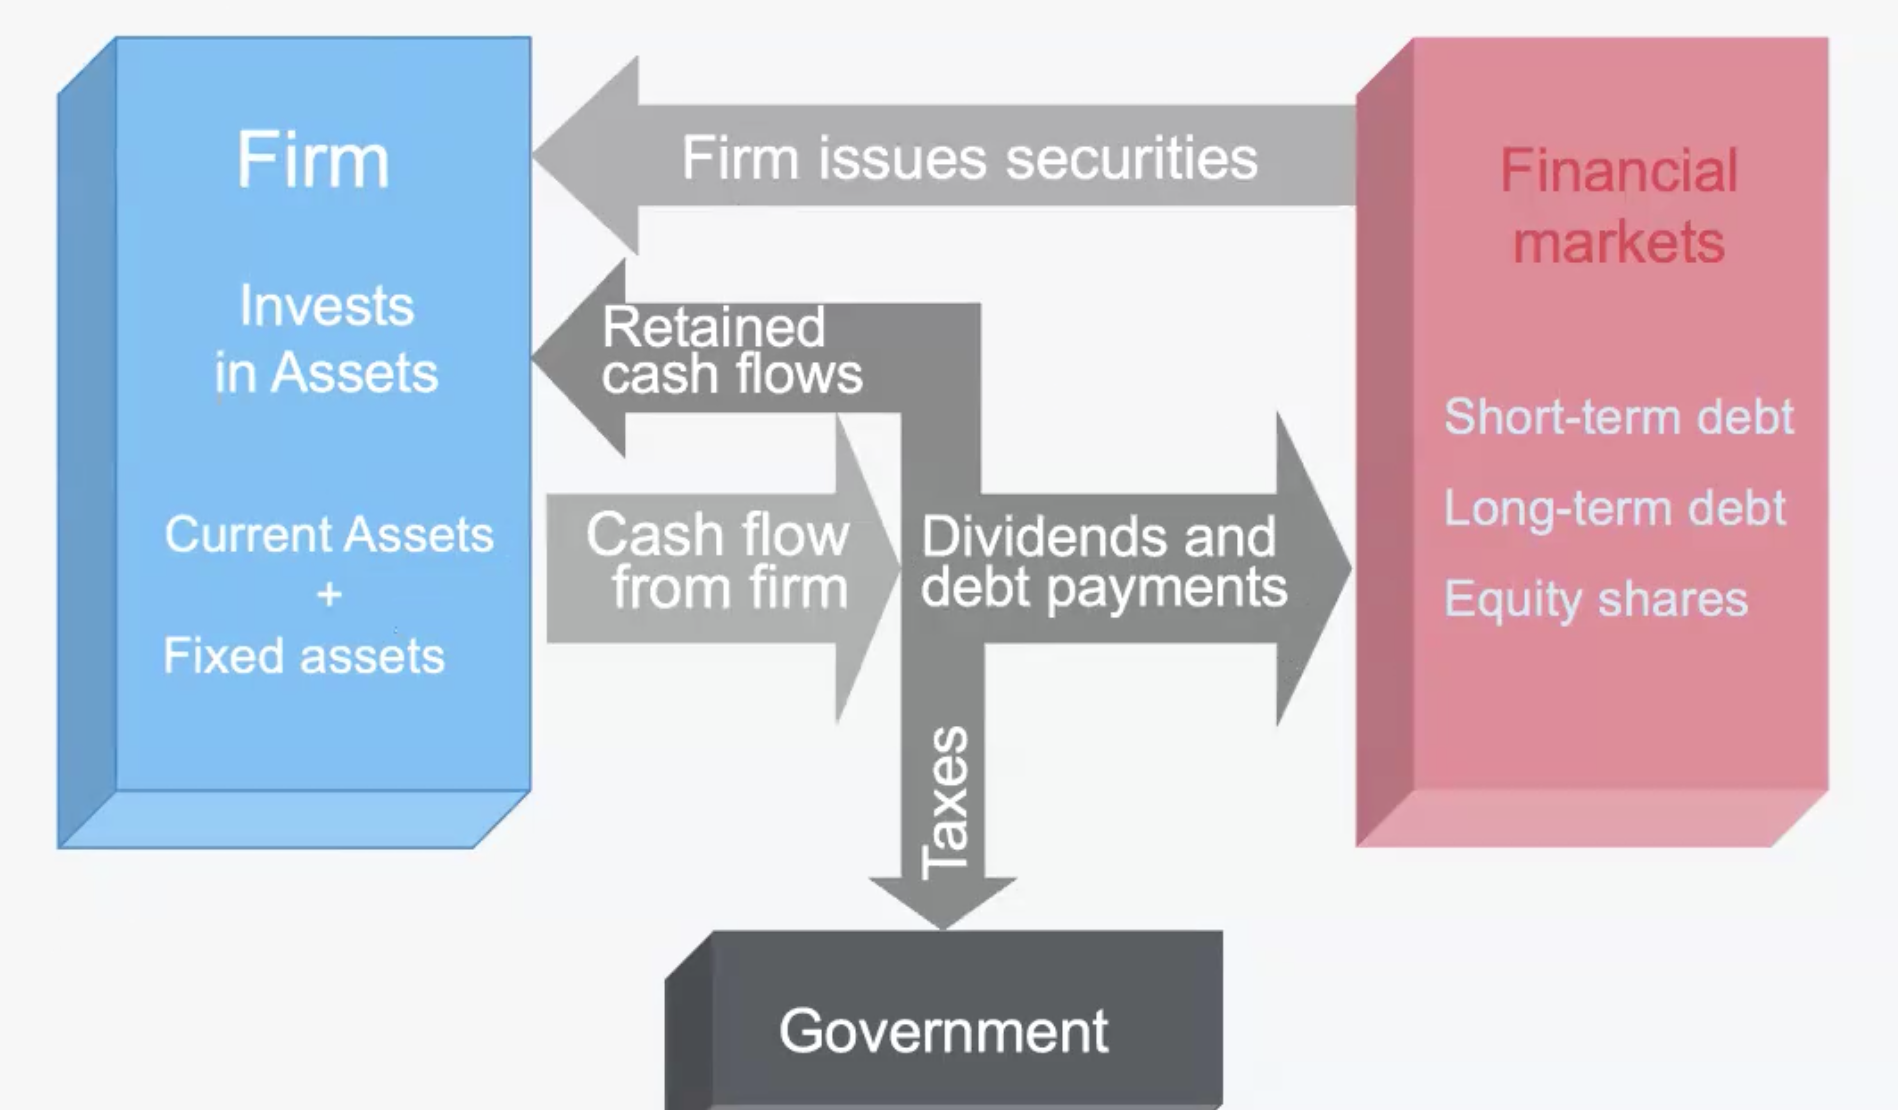
\includegraphics[width=0.8\textwidth]{img/2.2.png}
    \caption{The Role of Financial Markets}
\end{figure}

\begin{itemize}
    \item Company raises money to invest in assets through equity or debt.
    \item Equity or debt gets traded in the market.
    \item Company compensates investors with dividends or interest
    \item Company pays taxes to government
\end{itemize}

\subsection*{Yield Curves}
\begin{itemize}
    \item Term structure of interest rates, or the yield curve, is how zero-coupon bond yields change with bond maturity.
    \item When pricing bonds, we often assume a flat yield curve for simplicity. 
    \item This is not always the case, as they are generally upward sloping (but not always).
    \item Yield curve is usually represented by spot rates. A spot rate is the rate of interest on a bond with a single cash flow at a specific future date.
\end{itemize}

\begin{figure}[H]
    \centering
    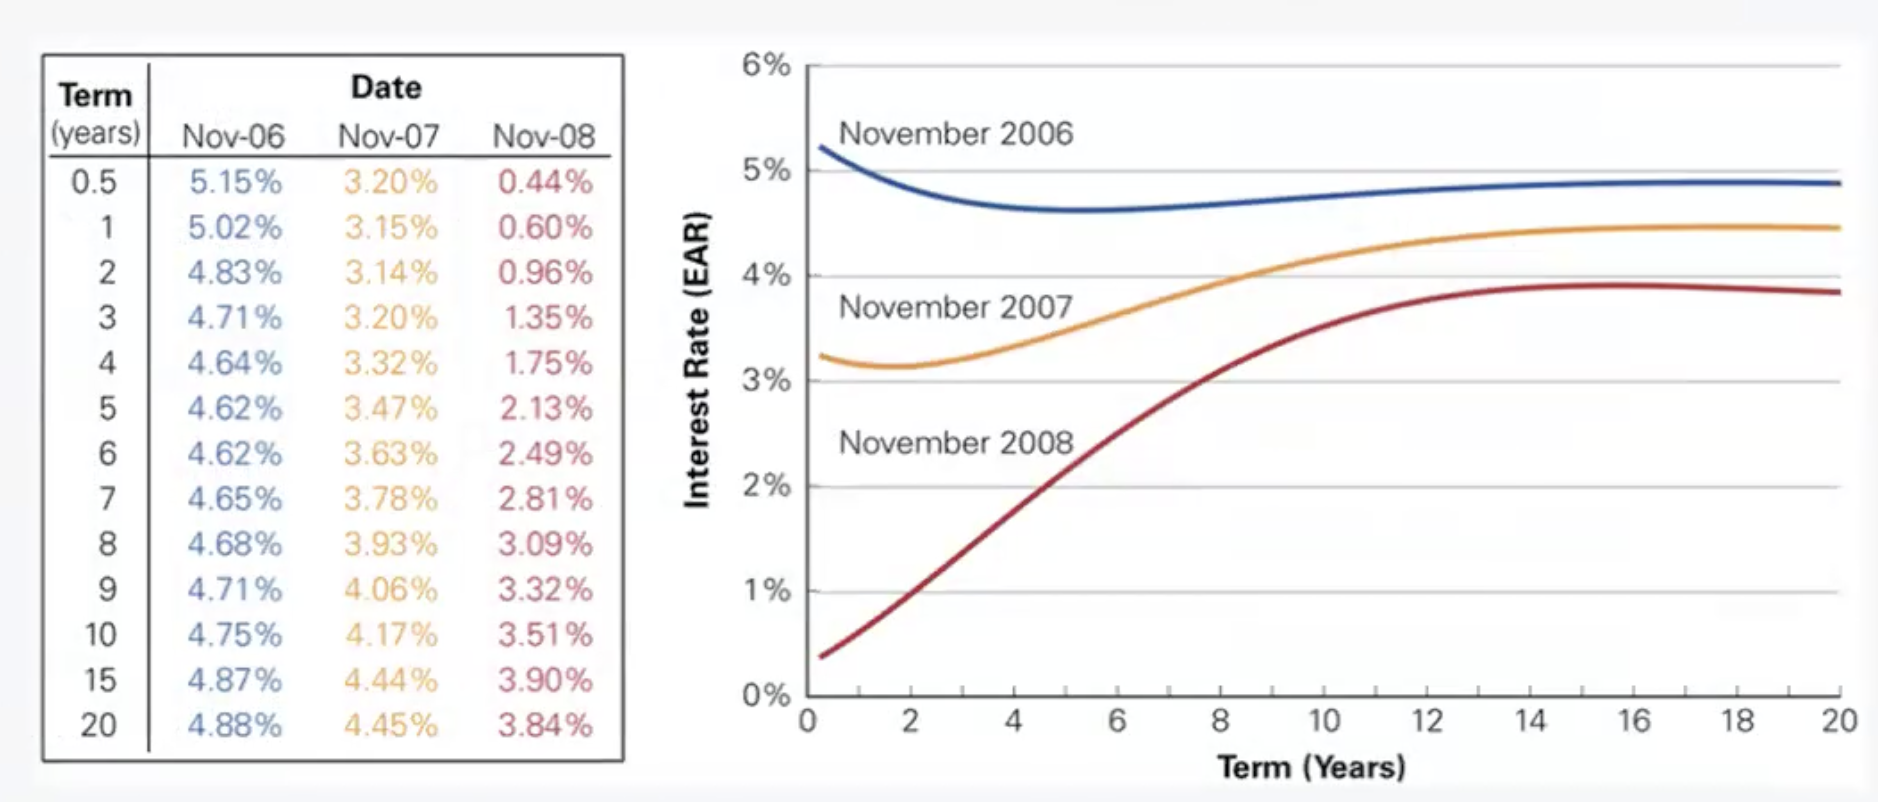
\includegraphics[width=0.8\textwidth]{img/2.3.png}
    \caption{Term Structure of Risk-Free U.S. Interest Rates, Nov 2006, 2007, 2008}
    \label{fig:term_structure}
\end{figure}
\begin{figure}[H]
    \centering
    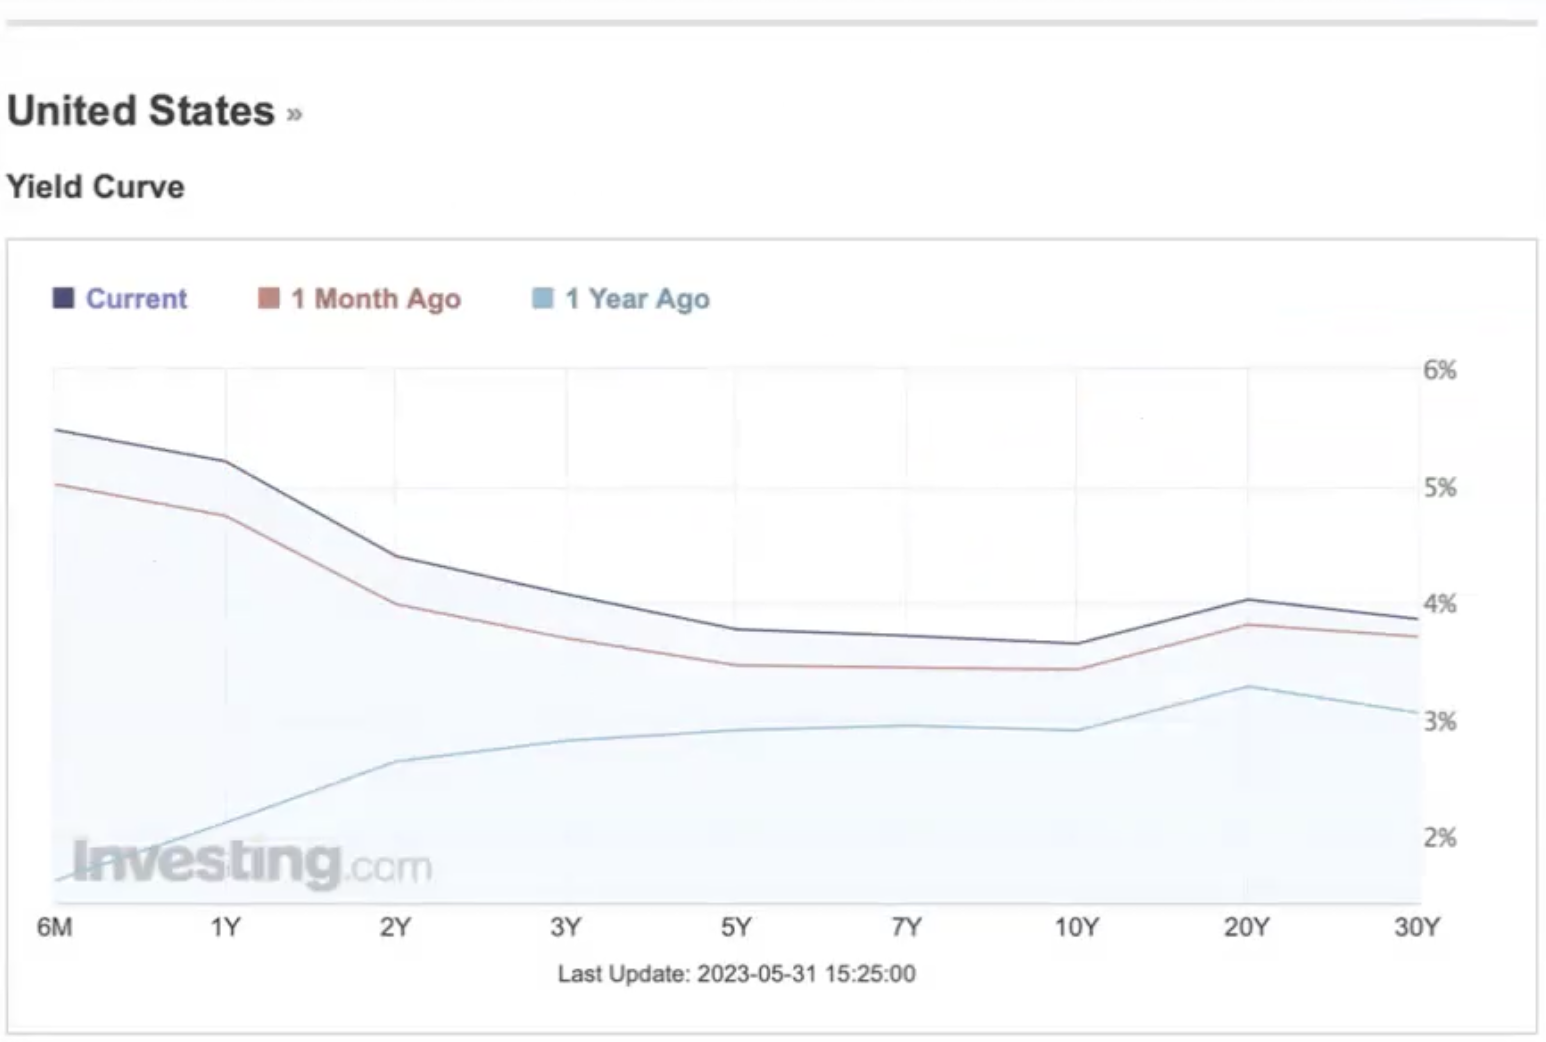
\includegraphics[width=0.8\textwidth]{img/2.4.png}
    \caption{Term Structure of Risk-Free U.S. Interest Rates, May 2023}
    \label{fig:term_structure2}
\end{figure}

From Figure \ref{fig:term_structure}, it can be seen that in November 2006 prior to the 2008 financial crisis, the yield curve was had relatively higher interest rates for the first two years, indicating an inverted yield curve which is a sign of an impending recession.\\

Similarly, in Figure \ref{fig:term_structure2}, the economy had an inverted yield curve in May 2023, despite a year ago having an upward sloping yield curve. 

\subsubsection*{Inverted Yield Curve as a sign of Recession} 
\begin{itemize}
    \item Normally, longer-term debt instruments should have a higher yield than shorter-term ones due to the increased risk of holding the bond for a longer period from inflation and the uncertainty of future interest rates.
    \item An inverted yield curve is when short-term debt instruments have a higher yield than longer-term ones. This is because investors expect future economic growth to slow, and that the central bank will have to lower interest rates to stimulate the economy.
    \item They are therefore then willing to accept lower yields on long-term bonds now, on the expectation that returns on future investments will be similarly low, if not lower. A long-term bond is generally a safer investment in times of economic uncertainty. 
    \item An inverted yield curve reduces the profitability of banks, as they borrow short-term and lend long-term, so the \textit{spread} between what banks can earn on long-term loans and what they pay on short-term borrowings decreases. This causes the bank to be more cautious in providing loans, leading to a reduction in lending, which can slow down the economy. 
    \item Furthermore, consumers expect interest rates to drop in the future (a common reason behind the inverted yield curve), and will postpone borrowing, also decreasing demand for loans in the short-term in banks. Conversely, if banks anticipate lower future interest rates, they will be less willing to offer long-term loans at current rates.
    \item Historically, an inverted yield curve has been a reliable indicator of an impending recession.
\end{itemize}

\subsection*{Spot Rates to Build Yield Curves}
Yield curves are built from spot rates, which are known today and start today. They are determined from yield to maturities on discount(zero-coupon) bonds, annualised for comparison purposes.\\

E.g. if I want to get a mortgage or a deposit, I check the spot rate for the term I want to borrow or lend for.\\

\begin{figure}[H]
    \centering
    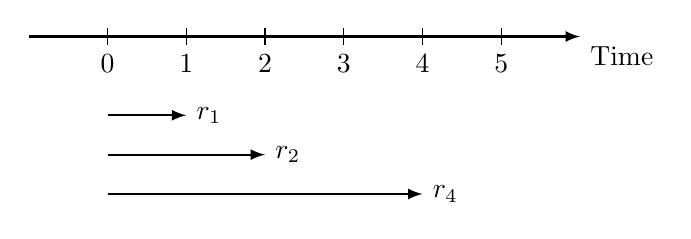
\begin{tikzpicture}
        % Draw the main number line
        \draw[thick, -latex] (-1,0) -- (6,0) node[anchor=north west] {Time};
        
        % Draw the spokes for 0-5
        \foreach \x in {0,...,5} {
          \draw (\x cm,3pt) -- (\x cm,-3pt) node[anchor=north] {$\x$};
        }
        
        % Draw the arrows for r1, r2, and r4
        \draw[thick, -latex] (0,-1) -- (1,-1) node[right, fill=white] {$r_1$};
        \draw[thick, -latex] (0,-1.5) -- (2,-1.5) node[right, fill=white] {$r_2$};
        \draw[thick, -latex] (0,-2.0) -- (4,-2.0) node[right, fill=white] {$r_4$};
    \end{tikzpicture}
    
\end{figure}

$r_1$ is the interest rate from time 0 to time 1, $r_2$ is the interest rate from time 0 to time 2, and so on.\\

\begin{examplebox}{Spot Rate Example Calculations}

\textbf{Question:} Suppose that a 5-year pure discount bond with face value \$100 is selling for \$95, what is the YTM on this bond?

\begin{align*}
    95 = \frac{100}{(1 + r_5)^5} \\
    (1+r_5)^5 = \frac{100}{95} \\
    r_5 = \left(\frac{100}{95}\right)^{\frac{1}{5}} - 1 = 1.031\%
\end{align*}

\end{examplebox}

\subsection*{Forward Rates}

The Bank of England website actually shows forward rates as default rather than spot rates. This is because the forward rate is the rate that you can lock in today as a loan or deposit for a future period.\\

\begin{itemize}
    \item Forward rates are interest rates set today for a future loan
    \item These rates are known today, but\textbf{ start in the future}
\end{itemize}


\begin{figure}[H]
    \centering
    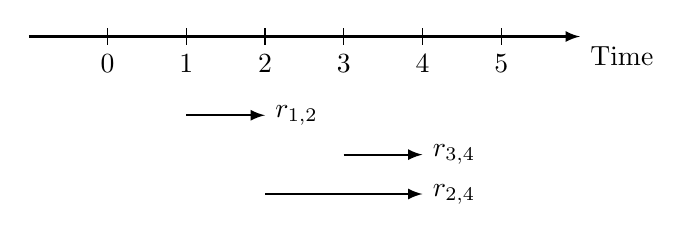
\begin{tikzpicture}
        % Draw the main number line
        \draw[thick, -latex] (-1,0) -- (6,0) node[anchor=north west] {Time};
        
        % Draw the spokes for 0-5
        \foreach \x in {0,...,5} {
          \draw (\x cm,3pt) -- (\x cm,-3pt) node[anchor=north] {$\x$};
        }
        
        % Draw the arrows for r1, r2, and r4
        \draw[thick, -latex] (1,-1) -- (2,-1) node[right, fill=white] {$r_{1,2}$};
        \draw[thick, -latex] (3,-1.5) -- (4,-1.5) node[right, fill=white] {$r_{3,4}$};
        \draw[thick, -latex] (2,-2.0) -- (4,-2.0) node[right, fill=white] {$r_{2,4}$};
    \end{tikzpicture}
    
\end{figure}

\begin{examplebox}{Forward Rate Example Calculations}
    Suppose we have the spot rates (forming an upwards yield curve) 3\% (1-year), 4\% (2-year), 5\% (3-year).
    What are the one-year forward rates?

    \begin{figure}[H]
        \centering
        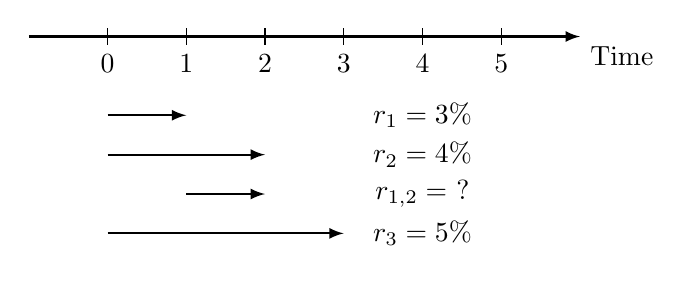
\begin{tikzpicture}
            % Draw the main number line
            \draw[thick, -latex] (-1,0) -- (6,0) node[anchor=north west] {Time};
            
            % Draw the spokes for 0-5
            \foreach \x in {0,...,5} {
              \draw (\x cm,3pt) -- (\x cm,-3pt) node[anchor=north] {$\x$};
            }
            
            % Draw the arrows 
            \draw[thick, -latex] (0,-1) -- (1,-1);
            \draw[thick, -latex] (0,-1.5) -- (2,-1.5);
            \draw[thick, -latex] (1,-2.0) -- (2,-2.0);
            \draw[thick, -latex] (0,-2.5) -- (3,-2.5);
            
            % Add labels
            \node at (4,-1) {$r_{1}=3\% $};
            \node at (4,-1.5) {$r_{2}=4\% $};
            \node at (4,-2.0) {$r_{1,2}= \ ?$};
            \node at (4,-2.5) {$r_{3}= 5 \% $};
        \end{tikzpicture}
        
    \end{figure}

    To get an intuitive idea for the forward rate calculation, we can say, if I am investing my money for a 2-year period (from years 0-2), this will be equivalent to investing for 1 year (from years 0-1), then reinvesting for another year (years 1-2) at the forward rate.


    \begin{align*}
        1.04^2 &= 1.03 \times (1 + r_{1,2}) \Rightarrow r_{1,2} = \frac{1.04^2}{1.03} - 1 = 5\%\\
        1.05^3 &= 1.04^2 \times (1 + r_{2,3}) \Rightarrow r_{2,3} = \frac{1.05^3}{1.04^2} - 1 = 7.03\% \\
               &= 1.03 \times 1.05 \times (1 + r_{2,3}) 
    \end{align*}


    Similarly:

    To find the forward rates, we can use the following relationships:

    \begin{align*}
        (1 + r_1)^1 &= (1 + r_1)(1 + r_{1,2}) \\
        (1 + r_2)^2 &= (1 + r_1)(1 + r_{1,2})(1 + r_{2,3}) \\
        (1 + r_3)^3 &= (1 + r_1)(1 + r_{1,2})(1 + r_{2,3})(1 + r_{3,4})
    \end{align*}

    Using these equations, we can solve for the forward rates:

    \begin{align*}
        (1 + 0.03)(1 + r_{1,2}) &= (1 + 0.04)^2 \\
        \Rightarrow\qquad r_{1,2} &= \frac{(1 + 0.04)^2}{(1 + 0.03)} - 1 = 5\%\\
        (1 + 0.04)^2(1 + r_{2,3}) &= (1 + 0.05)^3 \\
        \Rightarrow\qquad r_{2,3} &= \frac{(1 + 0.05)^3}{(1 + 0.04)^2} - 1 = 7.03\%
    \end{align*}


\end{examplebox}


\subsection*{Spot Rates in the Future - Theories}
There are three theories that try to explain and predict the yield curve:

\begin{itemize}
    \item Expectation Theory: The forward rate is the expected future spot rate. This is used in the calculation of forward rates.
    \begin{itemize}
                \item No risk premium: This theory assumes that investors do not demand a risk premium for holding long-term bonds, and that the forward rate is solely determined by the expected future spot rate.
                \begin{figure}[H]
                    \centering
                    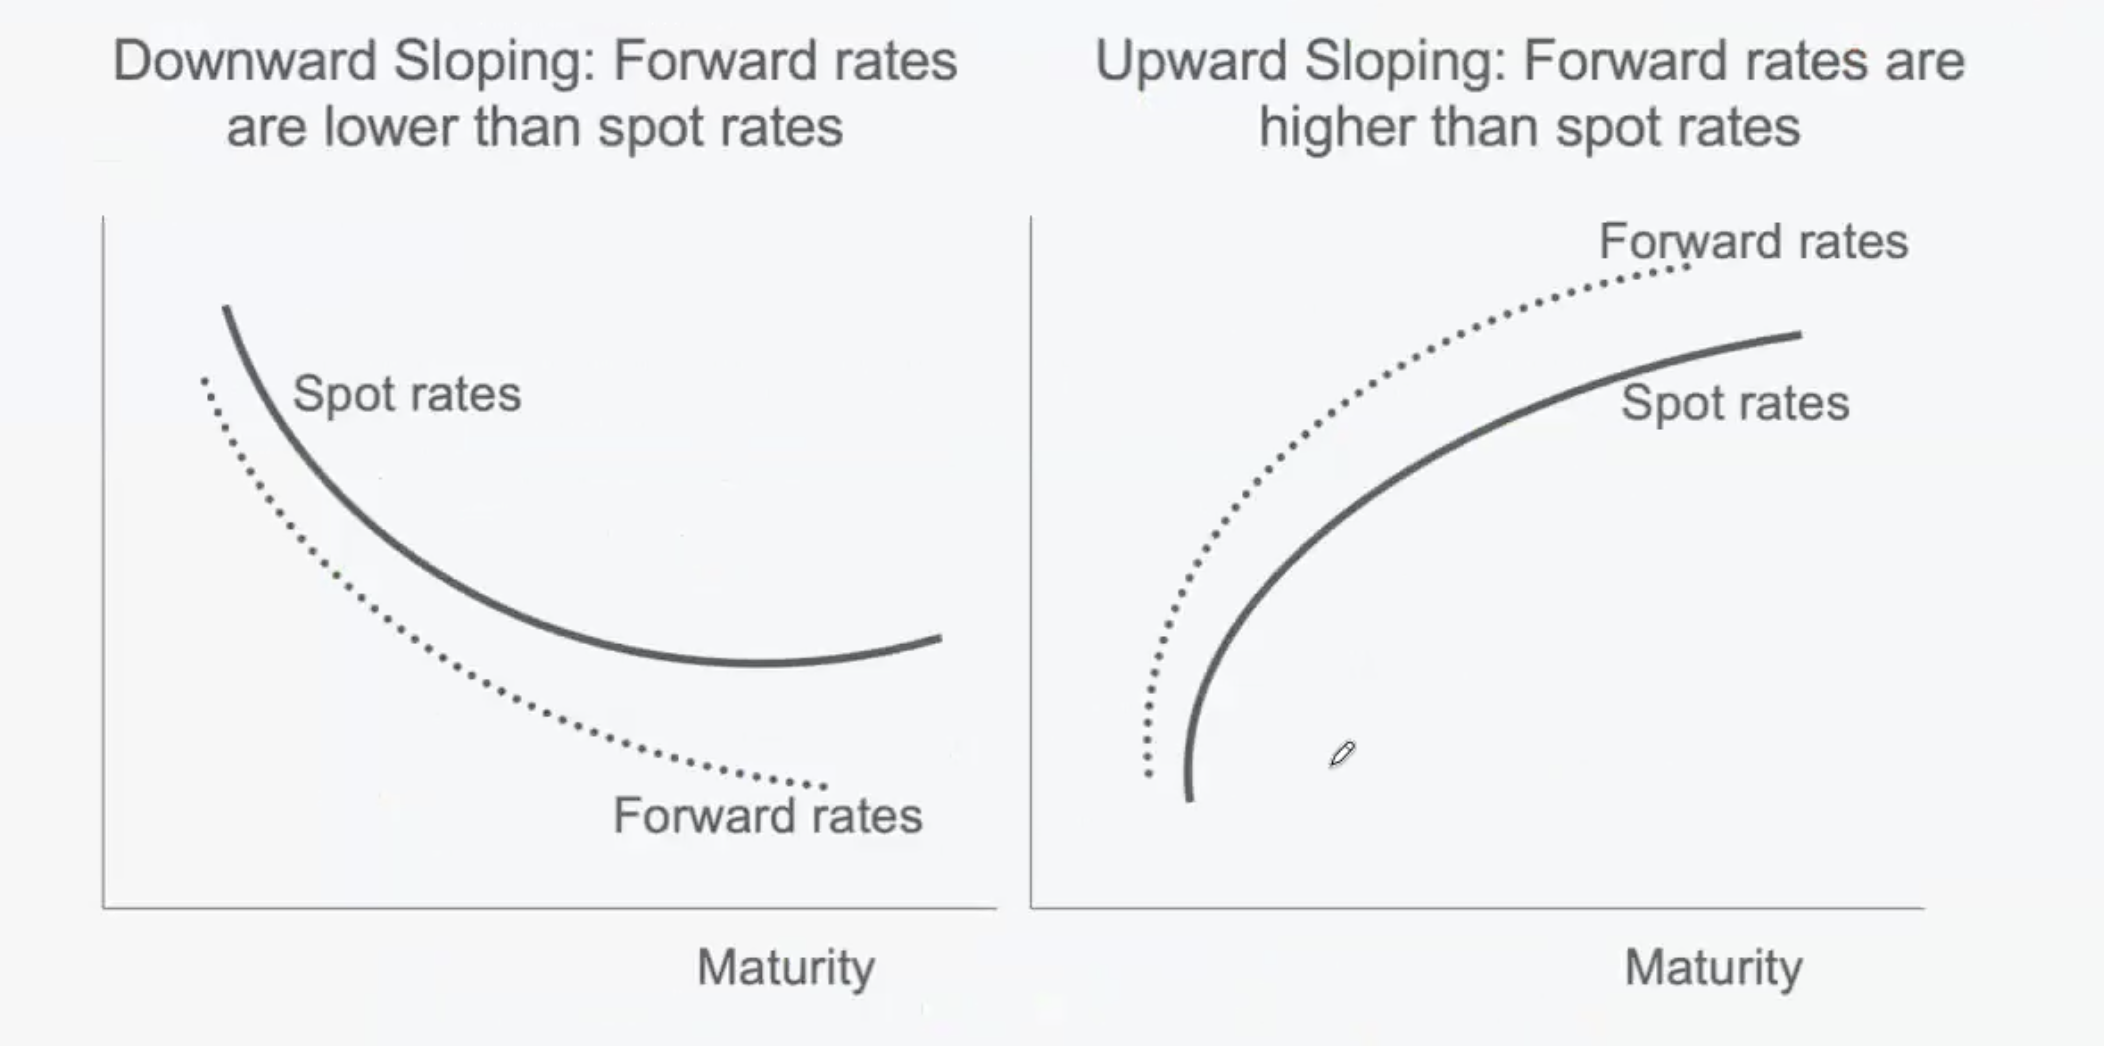
\includegraphics[width=0.8\textwidth]{img/2.5.png}
                \end{figure}
                \end{itemize}
    \item Liquidity Premium Theory:
    \begin{itemize}
                \item Long-term bonds are riskier than short-term bonds– This theory assumes that long-term bonds are riskier due to factors such as interest rate risk, credit risk, and liquidity risk.
                \item Investors demand a risk premium for holding long-term bonds: As a result, investors demand a higher return for holding long-term bonds, which leads to an upward-sloping yield curve.

    \end{itemize}
    \item Market Segmentation Theory:
    \begin{itemize}
                \item Bonds of different maturities are not substitutes: This theory assumes that bonds of different maturities are not perfect substitutes, and that investors have different preferences for bonds of different maturities.
                \item The supply and demand for bonds of each maturity determine the risk premium: The risk premium (and thus the yield curve) is determined by the supply and demand for bonds of each maturity, rather than by a single market-wide risk premium.
    \end{itemize}
\end{itemize}

\section{Corporate Bonds}
Prior to this section, government debt was discussed. Now this section focuses on corporate debt, which is more complex as corporations are potentially more likely to default than governments.

This is when a company fails to meet coupon payments, redemptions, or even financial distress such as liquidity shortages or going bankrupt. We rely on independent credit rating agencies like Moody's Fitch, and S\&P. They evaluate the quality of bonds based on credit quality assessing the likelihood of default over the bond's term. They provide qualitative ratings, for example, S\&P's:

\begin{itemize}
    \item AAA, AA, A, BBB: Investment Grade
    \item BB, B, CCC, CC, C: Speculative Grade
    \item D: Default
\end{itemize}

These ratings allow us to approximate the risk of default for a corporate bond. If a corporate bond has more credit risk (of default), investors will expect a higher yield to compensate for this risk. This is known as the credit spread, which is the difference between the yield on a corporate bond and the yield on a government bond of the same maturity.\\

The calculation of yield to maturity is similar as government debt, as the discount rate that equates the net present value of a bond's cash flow.

The credit ratings help use estimate average yield to maturity allowing us to plot yield curves for corporate bonds of varying risk levels and maturities.

\begin{figure}[H]
    \centering
    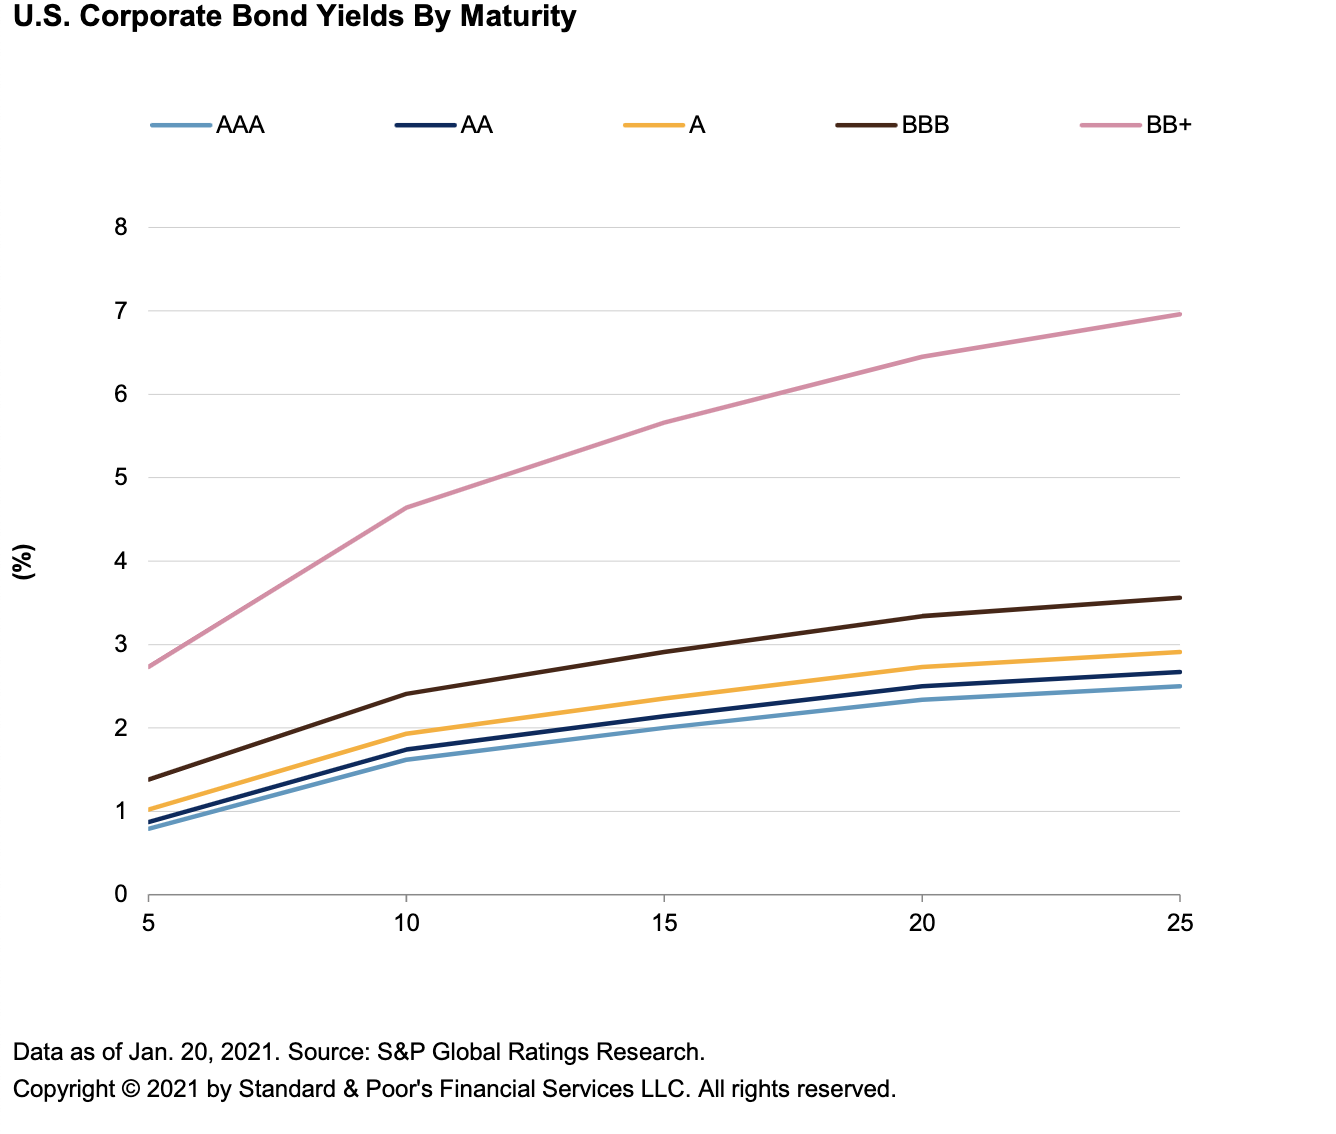
\includegraphics[width=0.5\textwidth]{img/2.6.png}
    \caption{Yield Curves for Corporate Bonds}
    \label{fig:corporate_yield_curve}
\end{figure}

In figure \ref{fig:corporate_yield_curve}, notice that moving down credit ratings, yields increase. The spread between the yields of corporate bonds serves as a gauge of credit risk. A wider spread indicates higher risk, with investors demanding higher yields to compensate for the increased risk of default.\\


\section{Green Bonds}
\begin{itemize}
    \item Green bonds are a financial instrument specifically to raise funds for environmentally-friendly projects, such as solar or wind farms, electric vehicle infrastructure or sustainable/efficient buildings.
    \item This allows investors to support projects that have a positive impact on the environment.
    \item Can be issue by governments, corporations, financial institutions, municipalities, banks, non-profits, and other entities.
    \item Can also be used to finance projects like reforestation, cleaning up or restoring habitats
\end{itemize}

\section{The Money Market}
\begin{sidenotebox}{The Money Market}

    \begin{itemize}
        \item Money markets offer \textbf{short-term, fixed-income instruments} with maturities of up to one year, facilitating the management of liquidity and short-term funding needs for firms, governments, and financial institutions.
        \item They function as a \textbf{large secondary market} for trading highly-liquid, short-term securities.
        \item Money markets provide a mechanism for entities to \textbf{manage surplus funds} efficiently and are a source of \textbf{low-cost short-term financing}.
        \item \textbf{Smaller investors} access these markets through \textbf{money market funds}, which are mutual funds that pool investors' funds to meet minimum capital requirements and achieve diversification.
        \item Unlike banks, which are \textbf{heavily regulated} and incur higher costs, money markets operate with \textbf{less regulatory oversight}, offering cost advantages especially in the trading of large sums.
    \end{itemize}
\end{sidenotebox}
    